%%%%%%%%%%%%%%
% To compile the latex source you the following packages
\documentclass[11pt,a4paper]{article}
\usepackage{color}
\usepackage{listings}
\usepackage{graphicx}
\usepackage{url}
\usepackage[ddmmyyyy]{datetime} 
\renewcommand{\dateseparator}{-}

\definecolor{bbb}{rgb}{.9,.9,.9}
\lstset{stepnumber=2, basicstyle=\small \ttfamily, language=matlab,
  frame=single, framerule=0.pt}

\usepackage[colorlinks=true, pdfstartview=FitV, linkcolor=blue,
citecolor=blue, urlcolor=blue]{hyperref}

\newcommand\kms{$\mathrm{km} \, \mathrm{s}^{-1}$}
\newcommand\kmsmath{\mathrm{km} \, \mathrm{s}^{-1}}



%%%%%%%%%%%%%%%%%%%%%%%%%%%%
%%%%%% Page dimensions %%%%%
%%%%%%  DO NOT CHANGE  %%%%%
%%%%%%%%%%%%%%%%%%%%%%%%%%%%

%\textheight=247mm
\textwidth=163mm
\topmargin=-7mm
\oddsidemargin=-10mm
\evensidemargin=-10mm
%\parindent 10pt

\setlength{\textwidth}{16.3cm}
\setlength{\oddsidemargin}{0cm}
\setlength{\evensidemargin}{0cm}
\addtolength{\textheight}{20mm}
\addtolength{\voffset}{-5mm}
\usepackage{sectsty}
\usepackage[small,bf,hang]{caption}

\allsectionsfont{\sffamily}
\chapterfont{\sffamily}
\chaptertitlefont{\sffamily}


%%%%%%%%%%%%%%%%%%%%%%%%%%%%%
%%%%% Start of document %%%%% 
%%%%%%%%%%%%%%%%%%%%%%%%%%%%%

\begin{document}
\pagestyle{plain}
\pagenumbering{arabic}
\title{\textsf{Reducing data from SALSA in \textsc{Matlab} -- {SalsaSpectrum}}}
\author{\textsf{Daniel Dahlin, Eskil Varenius}}
\yyyymmdddate
\date{\textsf{Revised: \today \, \currenttime}}
 

\maketitle

\section*{Abstract}
This document describes the use of the SalsaSpectrum \textsc{Matlab}
class, designed to assist when analysing data from the SALSA Onsala 
radio telescope. 

\tableofcontents

\section{Introduction}
\label{sec:introduction}

The SALSA Onsala telescope is a 2.3\,m in diameter antenna located at
Onsala space observatory outside Gothenburg. The telescopes are
designed to detect the faint radiation from cold hydrogen gas in our
galaxy, the Milky way. The hydrogen gas emits radiation at a
wavelength of 21 cm (or a frequency of 1420.4 MHz). This signal can be
detected by the microwave receiver connected to the telescope. 
The observed spectrum can be
exported into a FITS-file, which is the currently most used type of
file for astronomical images and spectra. The fits file has two parts:
(1) a \emph{header} which includes information
about the data such as the velocity resolution, central frequency and
many others, and (2) the data itself.

Having completed the observations, the observer may want to process
the data further in order to more accurately deduce the kinematics,
as well as the amount of hydrogen gas in the Milky Way. There are
currently two main options when analysing data from SALSA,
summarized here:

\begin{itemize}
\item \textbf{Salsa-J}: a software package that is used to reduce
  spectral data from the SALSA telscopes, but can also be used as a
  simple image editor and processor. A spectral module with
  functionality to reduce SALSA data is available. The main advantage
  of SalsaJ is its easy-to-use point-and-click interface. The main
  disadvantage is that reducing many spectra can be tedious. SalsaJ
  can be downloaded at the SALSA website. SalsaJ was developed for 
  the European Hands-On Universe (EU-HOU) project, an
  education project aimed to provide interesting exercises in the
  field of astronomy for high school students.
\item \textbf{SalsaSpectrum} is a data reduction environment written
  in the popular mathematical software \textsc{\textsc{Matlab}} -
  aimed for reduction of data from SALSA Onsala, developed by Daniel
  Dahlin.
\end{itemize}

There has previously not existed any published \textsc{Matlab} code to
handle data from SALSA (although several students have written their
own code over the years). This effort to write a Matlab class that
reads, reduces and analyzes data from SALSA was made to provide such a
code for use with \textsc{Matlab}. The class, named
\texttt{SalsaSpectrum} can be freely used, changed and improved by
anyone interested in the project. This document describes the use of
the \texttt{SalsaSpectrum} class at its current state.

\section{The SalsaSpectrum class}
\label{sec:salsaspectrum-class}

The code is implemented as a \textsc{Matlab} class. A fits-file from the SALSA
telescopes is read into memory as an object of the
\texttt{SalsaSpectrum} class. The user can then perform different
operations on the spectrum object, such as fitting a baseline, plot
the spectrum, calculate the noise level and fit a number of
gaussians to the spectrum. All results can be printed to screen and
the commands used to reduce the data can be placed in a \textsc{Matlab} m-file
for repeated use. It is also possible to write more complex scripts
and reduce many spectra at the same time.

The different capabilities of the \texttt{SalsaSpectrum} class will
now be presented.


\subsection{Installation}
\label{sec:installation}

The code used for the reduction environment is contained within one
\textsc{Matlab} m-file which includes the class definitions and functions. No
installation of the code is therefore needed. Move the m-file to the
directory where you do your work. \textsc{Matlab} will then automatically find
and use the \texttt{SalsaSpectrum} class.

If you want to use the class from many locations, you can store the
m-file in a central directory, and use the matlab \texttt{addpath}
command to add that location to the matlab path.

\begin{lstlisting}
  addpath /path/to/directory/with/SalsaSpectrum/class/files
\end{lstlisting}

\subsection{Read a spectrum}
\label{readaspectrum}

The class constructor method \texttt{SalsaSpectrum} is used to read a
spectrum from a fits-file and place it into the \texttt{SalsaSpectrum}
object \texttt{spec}

\begin{lstlisting}
  >> spec = SalsaSpectrum('Example/sample_data.fits')
\end{lstlisting}
If everything goes well the following information will be printed 
\begin{lstlisting}
>> spec

spec = 

  SalsaSpectrum handle

  Properties:
                    c: 299792458
               HIfreq: 1.4204e+09
              fittype: 0
             fileName: 'Example/sample_data.fits'
                 freq: [1x256 double]
                  vel: [1x256 double]
                index: [1x256 double]
                 info: [1x1 struct]
                 data: [1x256 double]
             baseLine: []
           baseWindow: []
     baseWindowParVel: []
     baseWindowParInd: []
    baseWindowParFreq: []
                  rms: []
             gaussFit: []
         gaussConfInt: []
             gaussPar: []
          gaussParVel: []
         gaussParFreq: []
             gaussErr: []
          gaussErrVel: []
         gaussErrFreq: []
      gaussIntegrated: []
            residuals: []
               labVel: []
               labSig: []
\end{lstlisting}

\noindent
Several properties of the object have already been added. Arrays
containing the data, info (the header), and frequency, velocity and
index have been created, as well as constants (the speeed of light and
the frequency of the HI line). Other properties are not yet
calculated. The functions that calculate and fill the empty variables are
discussed in the following sections.

\subsection{Plot a spectrum}
\label{sec:plot-spectrum}

It is easy to plot a spectrum. The \textsc{Matlab} class system allows two
types of calls to the plot function. A \texttt{SalsaSpectrum} object
\lstinline!spec! may be plotted either by using
\lstinline!spec.plot()! or \lstinline!plot(spec)!. Using these
commands on a SALSA spectrum results in the first graph shown in figure~\ref{fig1}.

\begin{figure}[h!]
  \centering
  \scalebox{0.55}{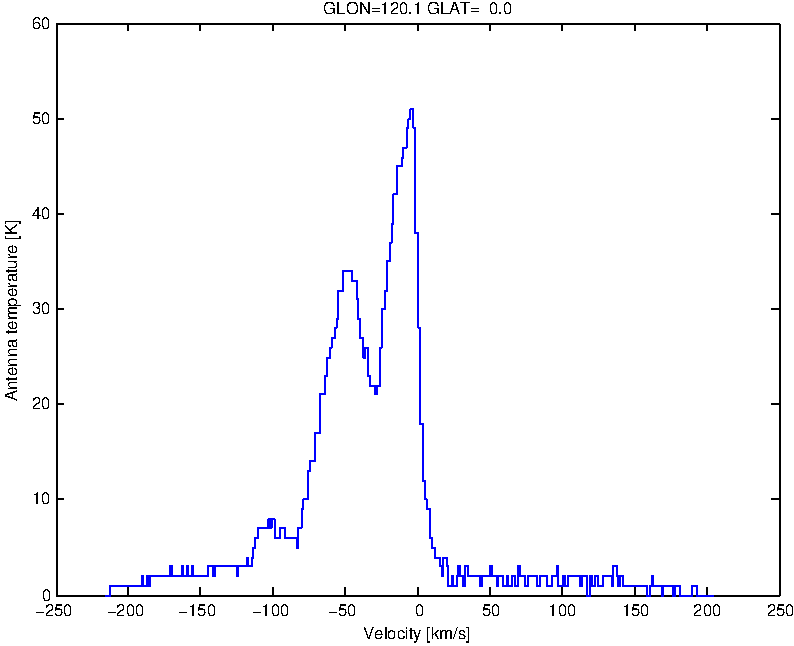
\includegraphics{figures/spec_vel}}
  \scalebox{0.55}{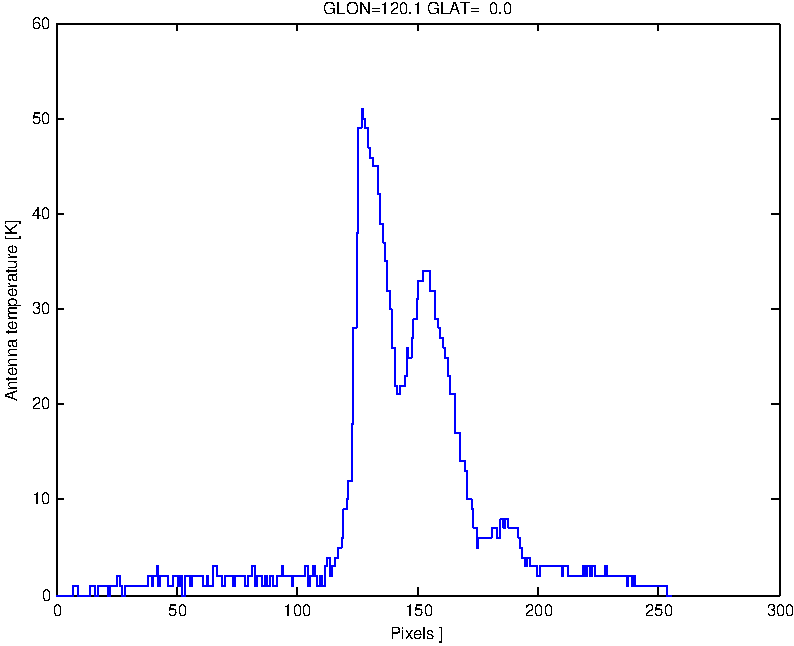
\includegraphics{figures/spec_pix}}
  \caption{Salsa spectra as a function of velocity and channel index
    (``pixel'').}
  \label{fig1}
\end{figure}

\noindent
The \texttt{plot} is an overloaded function, i.e. it has the same name
as the normal plot command but some extra features that makes the plot
more useful. A few such thing are apparent when looking at the
spectrum. The \texttt{SalsaSpectrum} class has made the decision to
display the spectrum as a function of velocity, which is the most
useful representation when working with a radioastronomical spectrum.
Labels are present for both axes. It is also possible to display the
spectrum as a function of frequency or channel index, by sending
either \texttt{'freq'} or \texttt{'pix'} to \texttt{plot}. An example
of a spectrum plotted in pixel scale is also shown in
figure~\ref{fig1}.

\subsection{Fit and subtract a baseline}
\label{sec:subtract-baseline}

In radioastronomical jargon, the ``baseline'' is the part of the
spectrum where no line emission is present. Spectra from SALSA are
produced by so-called \emph{frequency switching} which principally
removes any continuum signal that is present. However, the switching
technique is not perfect and sometimes a spectrum either is offset
from the zero-level, or has a small slope or parabola from one end to the
other. On such occasions it is customary to fit a baseline to the
spectrum. These principles are most easily understood when seeing an
example.

Fitting a baseline with \texttt{SalsaSpectrum} consists of finding the
spectral coordinates of the parts of the spectrum with no signal. The
end coordinates of that range are called \emph{spectral
  windows}. There are currently two ways of defining the spectral windows:
\begin{enumerate}
\item \emph{Manual method}: define spectral windows on the command
  line. Useful in scripts.
\item \emph{Interactive method}: define spectral windows using the
  mouse. 
\end{enumerate}
The two methods are described below in more detail.

\subsubsection{Manual method}
\label{sec:manual-method}

In the spectrum showed in Fig.~\ref{fig1} there is no signal between
velocities $+50$~\kms~and $+200$~\kms, or between, $-200$~\kms~and 
$-150$~\kms. The \texttt{fitBaseline}
command fits a polynomial to the data in the baseline windows. In the
following example, a polynomial of order $n=2$ (a parabola) is
fitted to the data in the spectral windows between $[-200~\kmsmath
\leq {v} \leq -150~\kmsmath]$ and $\left[ 50~\kmsmath \leq {v} \leq
  200~\kmsmath \right]$.
\begin{lstlisting}
>> spec.fitBaseline([ -200 -150 50 200],'vel',2)
\end{lstlisting}
\noindent
let us now take a look at the spectrum object again. 

\begin{lstlisting}
>> spec

spec = 

  SalsaSpectrum with properties:

                    c: 299792458
               HIfreq: 1.4204e+09
              fittype: 0
             fileName: 'Example/sample_data.fits'
                 freq: [1x256 double]
                  vel: [1x256 double]
                index: [1x256 double]
                 info: [1x1 struct]
                 data: [1x256 double]
             baseLine: [1x256 double]
           baseWindow: [1x123 double]
     baseWindowParVel: [-200.0828 -150.6162 50.5477 200.5962]
     baseWindowParInd: [246 216 94 3]
    baseWindowParFreq: [1.4214e+09 1.4211e+09 1.4202e+09 1.4195e+09]
                  rms: 0.7815
             gaussFit: []
         gaussConfInt: []
             gaussPar: []
          gaussParVel: []
         gaussParFreq: []
             gaussErr: []
          gaussErrVel: []
         gaussErrFreq: []
      gaussIntegrated: []
            residuals: []
               labVel: []
               labSig: []

\end{lstlisting}

The object has now been filled with more information related to the
baseline fit. The coefficients of the fitted polynomial, as well as
the actual polynomial as well the indices for the baseline windows in
all units have been added. Finally, the task has calculated the rms
value of the data in the baseline windows.

To show the fitted baseline, use the command \texttt{showBaseline}.
\begin{lstlisting}
>> spec.showBaseline()
\end{lstlisting}
which produces Fig. \ref{fig:baseline-fitted}.
\begin{figure}[h!]
  \centering
  \scalebox{1}{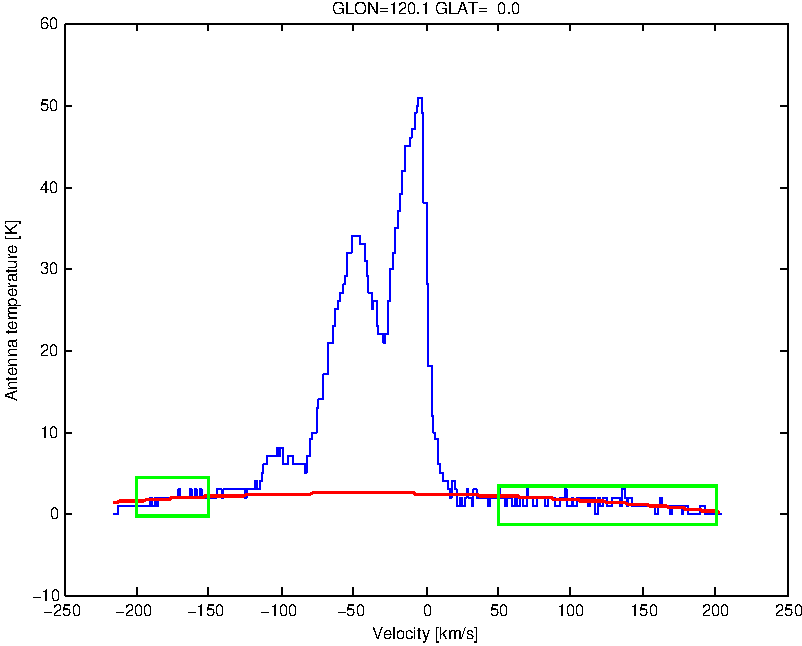
\includegraphics{figures/baseline_fitted}}
  \caption{Fitting a baseline. The \texttt{showBaseline} command
    produces this graph showing the fitted baseline as well as the
    baseline windows used for the fit. 
\label{fig:baseline-fitted}
}
\end{figure}

At this point, if you are satisfied with the baseline fit, you can
subtract the baseline from the spectrum with the function
\texttt{subtractBaseline}.
\begin{lstlisting}
>> spec.subtractBaseline()
\end{lstlisting}
In case you are not satisfied with the fit and want to change some
parameters, just redo the fit with new baseline windows or change the
order of the polynomial (as a rule-of-thumb, use $\mathtt{order}\leq3$
for good results). The new fit overwrites the previous one. Once you
are satisfied with the fit, use \texttt{subtractBaseline} to subtract
the baseline. A baseline-subtracted spectrum is shown in
Fig.~\ref{fig:baseline-subtracted}.
\begin{figure}[h!]
  \centering
  \scalebox{1}{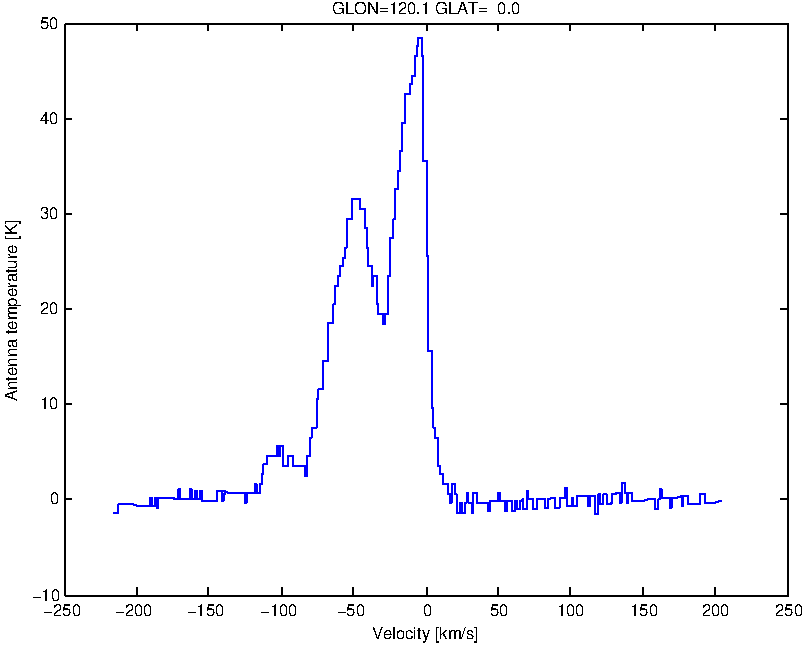
\includegraphics{figures/baseline_subtracted}}
  \caption{A baseline-subtracted spectrum plotted using
    \texttt{spec.plot()}.}
\label{fig:baseline-subtracted}
\end{figure}

It is not possible to subtract a baseline twice. 

\subsubsection{Interactive fit}
\label{sec:interactive-fit}

If you prefer to use the mouse to mark the baseline windows, you can
try the interactive method. Invoke the function
\texttt{fitBaseline} without arguments

\begin{lstlisting}
>> spec.fitBaseline()
\end{lstlisting}
\noindent
The following text is shown in the command window:

\begin{lstlisting}
   Mark each baseline window by clicking twice, on each side of the window.
   You can mark several windows but it is important that you only
   click an even number of times.
   Press return when you are finished.
\end{lstlisting}
\noindent
The baseline windows are then defined by marking the left and
rightmost channel of each window with the mouse. A crosshair appears
when the function is invoked. Left-click with the mouse to start
defining the baseline windows. Between pairs of points the color
changes, making it easier to see which pair a point belongs to. When
finished, press enter. After that, focus is given back to the command
window where you are asked to give the polynomial order. 

\begin{lstlisting}
   Input polynomial order: 2
\end{lstlisting}
\noindent
After that the same fitting routine is used as in the manual method. 

\begin{figure}[h!]
  \centering
  \scalebox{0.75}{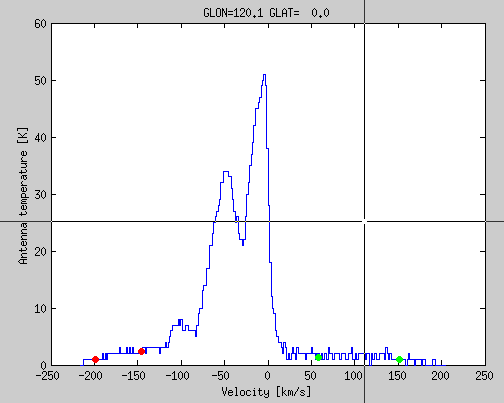
\includegraphics{figures/baseline_interactive.png}}
  \caption{Screenshot from interactive baseline fitting}
  \label{fig:interbaseline}
\end{figure}


\subsection{Fit gaussians to the spectrum}
\label{sec:fit-gauss-spectr}

The \texttt{fitGaussians} function fits up to five Gaussian functions
to the spectrum. There are (from version 1.7 of the code) three ways of
fitting gaussians to a spectrum:
\begin{enumerate}
\item \emph{Manual method}: supply starting guesses for the peak value,
  central velocity and
  velocity width of each gaussian function to be fitted. 
\item \emph{Blind fit}: allow the software to find peaks and fit
  Gaussians to them. This works well when the spectral lines are
  separated, but is not as good when fitting to blended lines.
\item \emph{Interactive fit}: mark peaks in the spectrum with the
  mouse and use those as starting guesses for the Gaussian fit. 
\end{enumerate}


\subsubsection{Manual method}
Starting guesses are entered in velocity units. The spectrum plotted in Figures
1, 2 and 3 appears to consist of three peaks at velocities about $-5$, $-50$
and $-100$~\kms, with intensities 50, 30 and 5.  Assuming an initial width of
10 ~\kms for each peak, the starting guesses for fitting three gaussian
profiles using the \texttt{fitGaussians} function would then be
\begin{lstlisting}
>> spec.fitGaussians([50 -5 10 30 -50 10 5 -100 10])
Fitting 3 Gaussians. 
Use plot() to see the fitted Gaussians.         
\end{lstlisting}
When the fit is completed, the spectrum object \texttt{spec} has been extended
with further parameters. 
\begin{lstlisting}
>> spec

spec = 

  SalsaSpectrum with properties:

                    c: 299792458
               HIfreq: 1.4204e+09
              fittype: 0
             fileName: 'Example/sample_data.fits'
                 freq: [1x256 double]
                  vel: [1x256 double]
                index: [1x256 double]
                 info: [1x1 struct]
                 data: [1x256 double]
             baseLine: [1x256 double]
           baseWindow: [1x90 double]
     baseWindowParVel: [-198.4339 -145.6696 58.7921 151.1297]
     baseWindowParInd: [245 213 89 33]
    baseWindowParFreq: [1.4213e+09 1.4211e+09 1.4201e+09 1.4197e+09]
                  rms: 0.5712
             gaussFit: [1x256 double]
         gaussConfInt: [1x512 double]
             gaussPar: [1x9 double]
          gaussParVel: [1x9 double]
         gaussParFreq: [1x9 double]
             gaussErr: [1x9 double]
          gaussErrVel: [1x9 double]
         gaussErrFreq: [1x9 double]
      gaussIntegrated: [1.0471e+03 1.3346e+03 113.9120]
            residuals: [1x256 double]
               labVel: []
               labSig: []
\end{lstlisting}
The parameters \texttt{gaussFit}, \texttt{gaussPar},
\texttt{gaussParVel} and \texttt{gaussParFreq} are now
non-empty. \texttt{gaussFit} is an array with the best-fit sum of
gaussians. The three other parameters hold the best-fit values for the
peak, central value and width of the gaussians.

The guesses should be quite close in order for the fit to be
good. When the fit is done the \texttt{spec.plot} command is used to show
the fitted gaussian functions.

\begin{figure}[h!]
  \centering
  \scalebox{0.7}{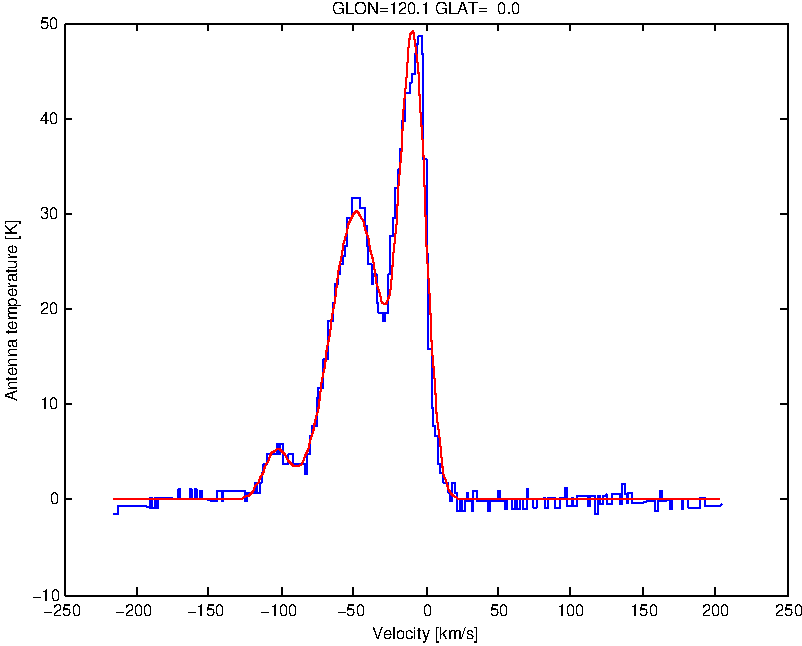
\includegraphics{figures/three_gauss_fitted.pdf}}
  \caption{Plot of a spectrum with three fitted gaussians overlaid.}
    \label{figGaussFit}
\end{figure}

\subsubsection{Automatic method}

The automatic method will search for peaks in the spectrum. It will
then fit Gaussians with the peaks as starting guesses for amplitude,
velocity center and width. To use the automatic method, call the
\texttt{fitGaussians} function without arguments.

\begin{lstlisting}
>> spec.fitGaussians()
\end{lstlisting}

An example of this fitting method is shown in Figure~\ref{fig6}. First
the automatic fit is applied, and three gaussians are found. However,
there is room for improvement at the negative velocities, so two extra
gaussians are manually added using the following syntax.

\begin{lstlisting}
>> spec.fitGaussians([guesses], 'dummy')
\end{lstlisting}

``Dummy'' could be number or string. This refits the previous
gaussians together with the new which can improve the total fit to the
spectrum. The parameter \texttt{guesses} has the exact same format as
in the manual fitting method, i.e. [\emph{Gauss peak 1}, \emph{Gauss
  center 1}, \emph{Gauss width 1}, \emph{Gauss peak 2} \ldots].

It is also possible to show the individual gaussians in a fit overlaid
on the spectrum. Call the \texttt{plot} function with the following
syntax.
\begin{lstlisting}
>> spec.plot('vel','individual')
\end{lstlisting}
where \texttt{'freq'} or \texttt{'pix'} could also be used. 

\begin{figure}[h!]
  \centering
  \scalebox{0.85}{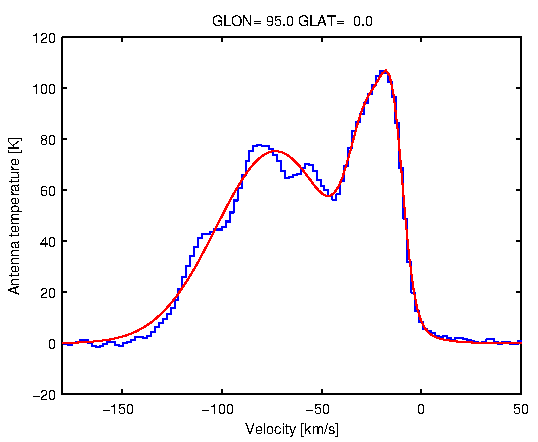
\includegraphics{figures/autogauss_step1}}
  \scalebox{0.85}{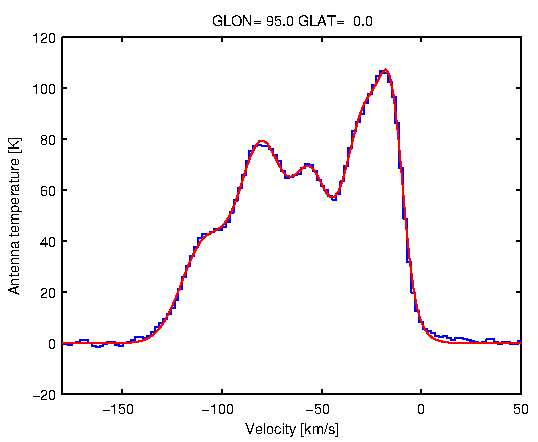
\includegraphics{figures/autogauss_step2}}
  \scalebox{0.85}{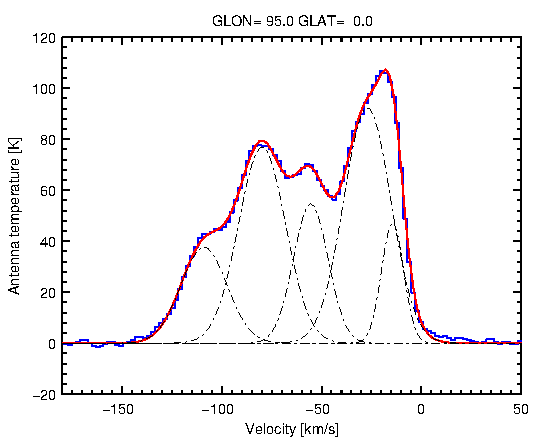
\includegraphics{figures/autogauss_step3}}
  \scalebox{0.85}{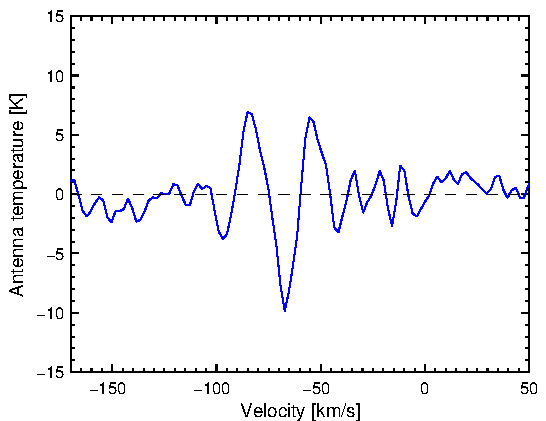
\includegraphics{figures/autogauss_step4}}
  \caption{Zoom-in on fit to blended spectrum. \emph{Top left}: blind
    fit. The algorithm cannot distuingish between the blended peaks
    between $-120$ and $-50$~\kms. \emph{Top right}: refining the
    blind fit by adding two additional gaussians. \emph{Bottom left}:
    same as top right, but also showing the individual gaussian
    functions. \emph{Bottom right}: residuals $\mbox{\emph{data}} -
    \mbox{\emph{Gaussian fit}}$ shown with the \texttt{showResiduals}
    function.}
  \label{fig6}
\end{figure}

\subsubsection{Interactive method}
\label{sec:interactive-method}

From version 1.7 of \texttt{SalsaSpectrum}, an interactive Gaussian
fit is included. It is designed as a wrapper around the
\texttt{fitGaussians} function, and it is called without arguments.
\begin{lstlisting}
>> spec.fitGaussiansInteractive()
\end{lstlisting}
When this function is invoked, the user can mark peaks in the
displayed spectrum with the mouse. Press the enter key when you are
finished marking the peaks. The data will then be sent to
\texttt{fitGaussians} which performs the actual fitting. An example is
shown in figure~\ref{fig:intergauss}.

\begin{figure}[h!]
  \centering
  \scalebox{0.75}{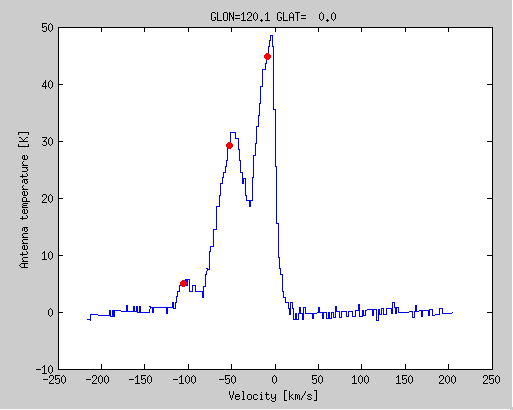
\includegraphics{figures/interactive_gaussian.png}}
  \caption{Screenshot from interactive Gaussian fitting.}
  \label{fig:intergauss}
\end{figure}

\subsubsection{Extracting fit parameters}
\label{sec:extr-fit-param}

After performing the gaussian fit, all fit parameters are available
within the \texttt{SalsaSpectrum} object. Of most interest to users is
probably the peak intensity of each Gaussian, their central velocity
and width. The integrated intensity of each gaussian is also
calculated.

Using the fit to the spectrum presented in figure~\ref{fig6} above,
the central velocities of the five gaussians are extracted with the
commands:
\begin{lstlisting}
>> spec.gaussParVel(1:3:end)  % peak of each gaussian
   47.6   92.5   77.0   54.8   37.7
>> spec.gaussParVel(2:3:end)  % central velocity of each gaussian
  -14.4  -27.0  -79.8  -55.4 -108.9
>> spec.gaussParVel(3:3:end)  % width (1sigma) of each gaussian
    5.5   11.9   11.8    8.7   11.5
\end{lstlisting}
and the integrated intensity:
\begin{lstlisting}
spec.gaussIntegrated
\end{lstlisting}

Uncertainties on the parameter values are calculated, and stored in
the \texttt{gaussErr}, \texttt{gaussErrVel} and \texttt{gaussErrFreq}
properties of the \texttt{SalsaSpectrum} object, when Gaussians have
been fitted. Finally, a 68\% confidence interval on the total sum of
Gaussians is calculated, and saved in the property
\texttt{gaussConfInt}. To visualize the confidence interval, use the
\texttt{showConfInt} function.
\begin{lstlisting}
>> spec.showConfInt()
\end{lstlisting}
which for the spectrum and Gaussian fit displayed in
Figure~\ref{figGaussFit}, produces the plot shown in
Figure~\ref{fig:confint}.

\begin{figure}[h!]
  \centering
  \scalebox{1}{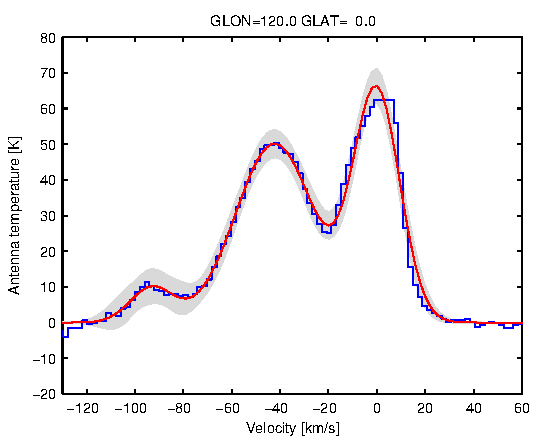
\includegraphics{figures/confint.pdf}}
  \caption{Spectrum with Gaussian fit and confidence intervals overlaid.}
  \label{fig:confint}
\end{figure}

\subsection{Saving your work}
\label{sec:saving-your-work}

A reduced spectrum can be saved so that the fitted baseline and
gaussians can be brought back later, without having to redo the
reduction. The built-in \textsc{Matlab} functions \texttt{save} and
\texttt{load} can be used to save and load a spectrum. To save the
spectrum stored in the object \texttt{spec1} to the
\textsc{\textsc{Matlab}} \texttt{.mat} file \texttt{spec1.mat}, simply
type:
\begin{lstlisting}
>> save spec1.mat spec1
\end{lstlisting}
This command places the .mat file spec1.mat in the current
directory. To read the file and bring back the SalsaSpectrum object,
type
\begin{lstlisting}
>> load spec1.mat
\end{lstlisting}
Note that to load a spectrum from a mat-file, the \texttt{SalsaSpectrum} class
must either be stored in the working directory, or added to the \textsc{Matlab}
path.

\subsection{Getting help}
\label{sec:getting-help}

Most of the functionality of \texttt{SalsaSpectrum} is described in
this manual. Online help is available in \textsc{\textsc{Matlab}} for several of the
functions, using the \texttt{help} syntax. Type \texttt{help
  functionName}. An example for the \texttt{fitBaseline}~function
follows.

\begin{lstlisting}
>> help fitBaseline
 --- help for SalsaSpectrum/fitBaseline ---

  fit a polynomial to the spectrum baseline. Define the
  baseline using a set of windows in the following way:
 
  [ x11 x12 x21 x22 x31 x32 ... ]
 
  as the first parameter passed to the function.
 
  check that the baseline vector consists of an even
  number of values.
 
   supply the baseline windows in units of
 
  1. indices     ['pix']
  2. velocity    ['vel']
  3. frequency   ['freq']
 
  by sending the string as a second argument. If you do not
  give any units, it is assumed that you have given indices.
 
  By default, this routine fits a first order polynomial
  to the chosen spectral windows. If you want another
  polynomial order, supply it as the third parameter.
 
  spec.fitBaseline([-200 -150 40 200], 'vel',2)
  
  will fit a second order polynomial between velocities -200
  to -150 and 40 to 200
\end{lstlisting}

\section{Cookbook}
\label{sec:cookbook}

How was the spectrum presented in figure~\ref{fig6}
reduced? Here are the steps summarized. This data
reduction is sufficient for most spectra.
\begin{lstlisting}
% read the spectrum
   spec=SalsaSpectrum('../SalsaFits/obs20060314/00031c.fits'); 
% fit a baseline
   spec.fitBaseline([-220 -150 30 220],'vel',3) 
% subtract the baseline
   spec.subtractBaseline() 
% perform blind gaussian fit
   spec.fitGaussians()
% refine the blind gaussian fit
   spec.fitGaussians([30 -55 6 30 -110 5], 'dummy') 
% read the LAB spectrum
   spec.readLab
% plot everything
   spec.plot; spec.showLab
\end{lstlisting}


\newpage
\section{Additional functions}
\label{sec:additional-function}

There is further functionality in the \texttt{SalsaSpectrum}~class
which are intended for more advanced users. They are listed here.

\subsection{Download data from the LAB survey}
\label{sec:download-data-from}

The LAB survey is a compilation of three major HI surveys performed
with telescopes in the Netherlands, Argentina and Australia. It covers
the entire sky and has a resolution of $30$ arcminutes. It can be
useful to compare the observed spectra taken with SALSA with those
from the LAB survey.

LAB spectra can be viewed and dowloaded at
\url{http://www.astro.uni-bonn.de/hisurvey/profile/}. The
high-resolution spectra can also be convolved to the resolution of the
SALSA telescopes ($\sim 5.4^{\circ}$ FWHM). The LAB data are available
for download as ascii-files.

\texttt{SalsaSpectrum} includes functionality so that the user can
automatically download and display a spectrum from LAB. The function
(\texttt{readLab}) downloads a spectrum at the coordinates of the
current spectrum. This function can be called for any
\texttt{SalsaSpectrum} object.

\begin{lstlisting}
>> spec.readLab
\end{lstlisting}

To reduce the use of the LAB server, the function also checks if the
appropriate data has already been downloaded. In figure~\ref{fig:lab}
a spectrum from SALSA toward the calibration region S7
($l=132^{\circ}$, $b=-1^{\circ}$) is compared to the LAB spectrum.

\begin{figure}[h]
  \centering
  \scalebox{1.2}{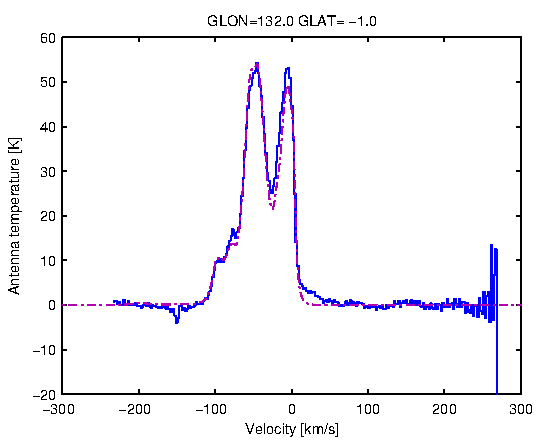
\includegraphics{figures/SALSA_vs_LAB.pdf}}
  \caption{SALSA spectrum taken toward S7 compared with the LAB
    spectrum, convolved to $5.4^{\circ}$ resolution.}
  \label{fig:lab}
\end{figure}

The spectra from LAB are presented in the brightness temperature
scale. The absolute calibration of data from SALSA is still
uncertain. There may therefore be differences between the LAB and
SALSA spectra due to calibration. 

\emph{Reference to the LAB survey}: Kalberla, P.M.W., Burton, W.B.,
Hartmann, Dap, Arnal, E.M., Bajaja, E., Morras, R., \& P\"{o}ppel,
W.G.L. (2005), A\&A, 440, 775


\subsection{Reduce several spectra}
\label{sec:reduce-sever-spectra}

The \texttt{SalsaSpectrum} class is easily extensible to allow
reduction of large sets of spectra from SALSA. If several fits files
from SALSA are stored in a directory, the following code will read
them and store them in the \textsc{Matlab} cell array \texttt{spec}. It also
fits baselines with different baseline windows depending on which 

% \textbf{Improvements}: I am planning to add functionality to the code
% so that baselines can be estimated automatically. It will also be
% possible to automatically estimate and fit gaussians to the spectrum. 

\begin{lstlisting}
direc = '/home/daniel/SalsaSpectra/SalsaFits/mwscan_l20l210/'
files = dir([direc,'*.fits']);

for i = 1:length(files)

    fname = [direc,files(i).name];
    spec{i} = SalsaSpectrum(fname);
    
    longspec(i) = spec{i}.getKeyword('CRVAL2');
    l = longspec(i);
        
    if (l>0 & l<40)
        spec{i}.fitBaseline([-240 -205 -140 -100 120 220],'vel',3);
    elseif (l>=40 & l<90)
        spec{i}.fitBaseline([-230 -200 -150 -110 100 220],'vel',3);
    elseif (l>=90 & l<180)
        spec{i}.fitBaseline([-230 -190 -130 -110 50 220],'vel',3);
    elseif l>=180
        spec{i}.fitBaseline([-230 -180 -120 -40 60 220],'vel',3);        
    end
    
    spec{i}.showBaseline()    
    spec{i}.subtractBaseline()
    spec{i}.fitGaussians()
    spec{i}.plot()  

end % end loop over spectra
\end{lstlisting}


\newpage

\section{List of functions and properties}
\label{sec:list-funct-param}

\subsection{List of properties}
\label{sec:list-properties}

\begin{lstlisting}[framerule=0pt]
    properties (Constant)
        c = 2.99792458e8;           % speed of light
        HIfreq = 1.42040575177e9;   % HI frequency in Hz
    end
    
    properties (GetAccess = 'private', SetAccess = 'private')
        baseSubtracted
        coordType
        gaussiansFitted
    end
    
    properties(GetAccess = 'public', SetAccess = 'private')
        % public read access, but private write access.
        fileName
    end
    
    properties
        freq                 % frequency array
        vel                  % velocity array
        index                % spectrum index array
        info                 % fitsinfo
        data                 % data spectrum
        baseLine             % fitted polynomial baseline
        baseWindow           % all indices of the baseline windows
        baseWindowParVel     % velocity values of start-end baseline window
        baseWindowParInd     % index values -"-
        baseWindowParFreq    % frequency values -"-
        rms                  % rms value calculated in the baseline windows
        gaussFit             % fitted gaussian functions
        gaussConfInt         % 68% confidence interval on the gaussian fit
        gaussPar             % parameters of gaussians
        gaussParVel          % -"- in velocity units
        gaussParFreq         % -"- in frequency units
        gaussErr             % 1 sigma errors on gaussians
        gaussErrVel          % -"- in velocity units
        gaussErrFreq         % -"- in frequency units
        gaussIntegrated      % integrated intensity in K km/s
        residuals            % residuals data - gauss fit
        labVel               % velocity axis of LAB spectrum
        labSig               % data of LAB spectrum        
    end % properties
\end{lstlisting}

\subsection{List of functions}
\label{sec:list-functions}

A complete list of the functions within the \texttt{SalsaSpectrum}
class follows, along with the information in each functions's help file.

\subsubsection*{SalsaSpectrum}
\label{sec:salsaspectrum}
\begin{lstlisting}[framerule=0pt]
  Class to initialize and do operations on spectra from the Salsa
  Onsala telescopes and the Qradio software. Create a spectrum object
  using the syntax
 
  spec = SalsaSpectrum('filename.fits');
 
  which then can be displayed and analyzed.
  
  
  This software comes with no warranty. It has been thoroughly
  tested, but there may still be bugs. It can be downloaded on the
  SALSA onsala Web site at brage.oso.chalmers.se , under "Salsa
  data in \textsc{Matlab}". 
  
  A manual describing how the class can be used is posted at together
  with this matlab class at
  http://brage.oso.chalmers.se/salsa/?q=node/142


\end{lstlisting}

\subsubsection*{plot}
\label{sec:plot}

\begin{lstlisting}[framerule=0pt]
  HANDLE = PLOT(obj,varargin)
  
  Plot a spectrum. The default syntax 
 
  spec.plot()
 
  By default the velocity scale is used. Other options are
  'pix' for indices and 'freq' for frequency.
 
  spec.plot('freq')
  
  If you have fitted Gaussians, they will also be
  displayed.
  
  If a second 'dummy' argument is supplied, and gaussians have
  been fitted, the individual Gaussians will be shown.
  
  spec.plot('vel', 'dummy')
\end{lstlisting}

\subsubsection*{showResiduals}
\label{sec:showresiduals}

\begin{lstlisting}[framerule=0pt]
  SHOWRESIDUALS(obj)
  
  Plot the residuals; the difference between the data and
  the Gaussian model. 
\end{lstlisting}

\subsubsection*{showIndividual}
\label{sec:showindividual}

\begin{lstlisting}[framerule=0pt]
  HANDLE = SHOWINDIVIDUAL(obj,varargin)
  
  plots the individual gaussian functions fitted to the spectrum. Can
  only be called after fitGaussians has ben used.            
\end{lstlisting}

\subsubsection*{shiftVel}
\label{sec:shiftvel}

\begin{lstlisting}[framerule=0pt]
  SHIFTVEL(obj,deltav)
  
  Shift the velocity scale by a value. To shift the scale 20 km/s
  toward positive velocities, use
  
  spec.shiftVel(-20)
\end{lstlisting}

\subsubsection*{scale}
\label{sec:scale}

\begin{lstlisting}[framerule=0pt]
  SCALE(obj,scalefac)
  
  Scale the spectrum and fitted Gaussians by a factor, by
  multiplication. To scale a spectrum down by 20 percent, use the
  command
  
  spec.scale(8/10)
\end{lstlisting}

\subsubsection*{fitBaseline}
\label{sec:fitbaseline}

\begin{lstlisting}[framerule=0pt]
  FITBASELINE(obj,varargin)
  
  fit a polynomial to the spectrum baseline. Define the
  baseline using a set of windows in the following way:
 
  [ x11 x12 x21 x22 x31 x32 ... ]
 
  as the first parameter passed to the function.
 
  The baseline vector should consist of an even number of
  values. If not, the function gives an error.
 
  The baseline windows are supplied in units of
 
  1. indices     ['pix']
  2. velocity    ['vel']
  3. frequency   ['freq']
 
  Send the string (e.g. 'vel') as a second argument. The index
  unit is default.
 
  By default, this routine fits a first order polynomial to
  the chosen spectral windows. Supply another polynomial order
  as an argument
 
  spec.fitBaseline([-200 -150 40 200], 'vel', 2)
  
  This command will fit a second order polynomial between
  velocities -200 to -150 and 40 to 200
\end{lstlisting}

\subsubsection*{getIndices}
\label{sec:getindices}

\begin{lstlisting}[framerule=0pt]
  help function for the fitBaseline function
\end{lstlisting}

\subsubsection*{showBaseline}
\label{sec:showbaseline}

\begin{lstlisting}[framerule=0pt]
  SHOWBASELINE(obj) 
  Show the fitted baseline overlaid on the spectrum, as well as boxes
  indicating the baseline windows. 
  
  spec.showBaseline() 
  
  This function does not subtract the baseline. Use the
  subtractBaseline function to do that.
\end{lstlisting}


\subsubsection*{subtractBaseline}
\label{sec:subtractbaseline}

\begin{lstlisting}[framerule=0pt]
  SUBTRACTBASELINE(obj)
  
  Subtract the fitted baseline from the data.
\end{lstlisting}


\subsubsection*{fitGaussians}
\label{sec:fitgaussians}

\begin{lstlisting}[framerule=0pt]
  FITGAUSSIANS(obj,varargin)    
  Fit a number of gaussians to the spectrum. Supply guess
  values of height, central value and width of each
  gaussian, in units of velocity.
  
  spec.fitGaussians([60 0 8 30 -55 10])                
                 
  If you don't supply any guess, the function will search
  for peaks in the spectrum and use those as starting
  guesses for the fit. If the fit is not good, you can
  redo it with a new guess.
 
  If you want to add gaussians to a fit, call this
  function again with guesses for the new gaussian, and
  send a second dummy argument, like
 
  spec.fitGaussians([60 -10 10],'dummy')
 
  which will add an extra gaussian of peak 60 K, central
  velocity -10 km/s and velocity width 10 km/s to the fit.
\end{lstlisting}


\subsubsection*{getRms}
\label{sec:getrms}

\begin{lstlisting}[framerule=0pt]
  GETRMS(obj)
  
  calculate and display the rms of the data contained in the baseline
  windows.
\end{lstlisting}


\subsubsection*{showBaselineWindows}
\label{sec:showbaselinewindows}

\begin{lstlisting}[framerule=0pt]
  SHOWBASELINEWINDOWS(obj)
  
  Plot a graphical representation of the chosen
  baseline windows.
\end{lstlisting}


\subsubsection*{getKeyword}
\label{sec:getkeyword}

\begin{lstlisting}[framerule=0pt]
  GETKEYWORD(OBJ, KEY) returns the value of KEY from the fits
  header OBJ.INFO.  
  
  This function was kindly provided by Magnus Sandén and Eskil
  Varenius.
\end{lstlisting}


\subsubsection*{showLab}
\label{sec:showlab}

\begin{lstlisting}[framerule=0pt]

\end{lstlisting}


\subsubsection*{readLab}
\label{sec:readlab}

\begin{lstlisting}[framerule=0pt]
  READLAB(obj)
  
  download data from the LAB survey at
  http://www.astro.uni-bonn.de/hisurvey/profile/index.php
  
  convolved to Salsa's angular resolution
\end{lstlisting}

\subsubsection*{clipSpectrum}
\label{sec:clipspectrum}

\begin{lstlisting}[framerule=0pt]
  BACK = CLIPSPECTRUM(obj,window)
  
  NOTE: EXPERIMENTAL, USE AT YOUR OWN RISK.
  
  given the indices in the window parameter, this
  function "clips" (removes) the indicated spectral
  channels from the data. Several spectral windows can
  be specified.  Only the 'pixel' spectral unit can be
  used. 
  
    spec.clipSpectrum([1 10 230 250])
  
  would clip all channels between channels 1 and 10 (1 2 3
  4 5 6 etc) and between channels 230 and 250.
\end{lstlisting}

\subsubsection*{despike}
\label{sec:despike-1}

\begin{lstlisting}[framerule=0pt]
  DESPIKE(obj,varargin)
          
  NOTE: EXPERIMENTAL, USE AT YOUR OWN RISK.
  
  experimental function to remove 'spikes' in the data. Works well for
  the spike at the edge of the spectrum, works
  sometimes also for strong RFI in the spectrum.
\end{lstlisting}

\subsubsection*{smoothSpectrum}
\label{sec:smoothspectrum}

\begin{lstlisting}[framerule=0pt]
  SMOOTHSPECTRUM(obj,varargin)
  
  Smooth a spectrum to a lower spectral resolution. To lower
  the resolution by a factor of 2, supply the command
  
  spec.smoothSpectrum(2)
\end{lstlisting}


\section{Changelog}
\label{sec:changes}
Change log for this document. Code changes are described in the code.

\vspace{2ex}
\noindent 
\emph{version 1.91}
\begin{itemize}
\item 2014-12-27: Uploaded this document to the SALSA github repository to
track future changes. Also replaced some figures using data from the new
software defined radio receiver system, and did some minor text changes.
\end{itemize}
\vspace{2ex}
\noindent 
\emph{version 1.9}
\begin{itemize}
\item 2014-12-26: Small changes to the text.
\end{itemize}
\vspace{2ex}
\noindent 
\emph{version 1.8}
\begin{itemize}
\item Rewrote the \texttt{readLab} function so that it now also works
  on Windows machines. 
\end{itemize}
\vspace{2ex}
\noindent
\emph{version 1.7}
\begin{itemize}
\item Added information about interactive fitting of baselines and
  Gaussians
\end{itemize}
\vspace{2ex}
\noindent
\emph{Version 1.6}
\begin{itemize}
\item added documentation for all functions
\item tidied up the document
\end{itemize}
\vspace{2ex}
\emph{Version 1.3}
\begin{itemize}
\item Major reorganisation of the text
\item added figures and examples
\end{itemize}
\vspace{2ex}
\noindent\emph{Version 1}
\begin{itemize}
\item Initial documentation
\end{itemize}
\vspace{2ex}





\section{Conclusions and outlook}
\label{sec:conclusion-outlook}

This document is a brief manual in the use of the
\texttt{SalsaSpectrum} \textsc{Matlab} class. The manual is intended to reflect
the methods available in the \textsc{Matlab} class. However, it is possible
that this documentation will lag the code itself. My hope is that the
code will be useful for some people interested in reducing data from
SALSA.\\

\hfill G{\"o}teborg, March 11, 2013\\

\hfill \emph{Daniel Dahlin}

\end{document}

